\documentclass[10pt, conference]{IEEEtran} %compsocconf
\usepackage{graphicx}

%\usepackage{algorithmic}
\usepackage{algorithm}
\usepackage[noend]{algpseudocode}
\usepackage{array}
\usepackage{amsfonts}
\usepackage{graphicx}
\usepackage{epstopdf}
\usepackage{amssymb}
\usepackage{tikz,pgfplots}
\usetikzlibrary{snakes,arrows,shapes,trees}
\usepackage[position=top,aboveskip=5pt,labelformat=empty]{subfig}
\usepackage{xcolor, graphicx}
\usepackage{amssymb,amsmath,amsthm}
\usepackage{amsopn}
\usepackage{listings}
\usepackage{adjustbox}
\usepackage{longtable}
\usepackage{multirow}
%\usepackage{subcaption}
\DeclareMathOperator{\diag}{diag}

\usepackage{minted}
%\usepackage[outputdir=build]{minted}
\usepackage{amssymb}
\usepackage{pgfplots}
\usepackage{pgfplotstable}
\usetikzlibrary{arrows,shapes,plotmarks}
\pgfplotsset{compat=1.8}

\usepackage{soul}

\usepackage[pdfinfo={Title={Massively Parallel Simulations of Binary Black Hole Intermediate Mass Ratio Inspirals},Subject={SC'18 Applications Paper},Author={Anonymous},pKeywords={Computational Relativity,Einstein Equations,Adaptive Mesh Refinement,Finite Differencing,Wavelet Adaptive Multiresolution}},bookmarks=false,colorlinks=true,urlcolor=darkgray,linkcolor=darkgray,citecolor=violet]{hyperref}

% correct bad hyphenation here
\hyphenation{op-tical net-works semi-conduc-tor}

\definecolor{bgblue}{RGB}{245,243,253}

%\newcommand{\Summit}{\href{https://www.olcf.ornl.gov/summit/}{Summit}}
%\newcommand{\Aurora}{\href{http://aurora.alcf.anl.gov/}{Aurora}}
%\newcommand{\Stampede}{\href{https://www.tacc.utexas.edu/stampede/}{Stampede}}
%\newcommand{\Titan}{\href{https://www.olcf.ornl.gov/titan/}{Titan}}

\newcommand{\mynote}[3]{
    \textcolor{#2}{\fbox{\bfseries\sffamily\scriptsize#1}}
        {\small$\blacktriangleright$\textsf{\emph{#3}}$\blacktriangleleft$}
}


\def\TT{{T}}
\def\SS{{step}}

\newcommand{\dn}[1]{\mynote{David}{magenta}{#1}}
\newcommand{\mf}[1]{\mynote{Milinda}{blue}{#1}}
\newcommand{\hs}[1]{\mynote{Hari}{olive}{#1}}
\newcommand{\ewh}[1]{\mynote{Eric}{red}{#1}}

\newcommand{\dendro}{\textsc{Dendro}}
\newcommand{\NLSM}{\textsc{NLSM}}
\newcommand{\dendrogr}{\textsc{Dendro-GR}}
\newcommand{\HAD}{\textsc{Had}}
\newcommand{\et}{\textsc{ET}}
\newcommand{\bsolver}{\texttt{bssnSolver}}
\newcommand{\BSSN}{BSSNKO}


\newcommand{\oTo}{\textsc{o2o}}
\newcommand{\oTn}{\textsc{o2n}}

\newcommand{\subsubsubsection}[1]{\paragraph{#1}\mbox{}}
\setcounter{secnumdepth}{4}
\setcounter{tocdepth}{4}



\theoremstyle{plain}
\newtheorem{thm}{Theorem}[section]
\newtheorem{lem}[thm]{Lemma}
\newtheorem{prop}[thm]{Proposition}
\newtheorem*{cor}{Corollary}

\theoremstyle{definition}
\newtheorem{defn}{Definition}[section]
\newtheorem{conj}{Conjecture}[section]
\newtheorem{exmp}{Example}[section]

\theoremstyle{remark}
\newtheorem*{rem}{Remark}
%\newtheorem*{note}{Note}

\pgfplotsset{compat=1.13}

\hyphenation{op-tical net-works semi-conduc-tor}

%% user command
\newcommand{\mvec}{\textsc{matvec}}
\newcommand{\tsort}{\textsc{TreeSort}}
\newcommand{\tsearch}{\textsc{TreeSearch}}
\newcommand{\tcons}{\textsc{TreeConstruction}}
\newcommand{\dtcons}{\textsc{DistTreeConstruction}}
\newcommand{\taux}{\textsc{AuxiliaryOctants}}
\newcommand{\tbal}{\textsc{TreeBalancing}}
\newcommand{\tdbal}{\textsc{DistTreeBalancing}}
\newcommand{\tghost}{\textsc{ComputeGhostOctants}}
\newcommand{\teToe}{\textsc{BuildOctantToOctant}}
\newcommand{\teTon}{\textsc{BuildOctantToNodal}}

\newcommand{\hilbertcurve}{\textsc{Hilbert}}
\newcommand{\mortoncurve}{\textsc{Morton}}

\newcommand{\dgn}{\textit{octant local nodes}}
\newcommand{\cgn}{\textit{shared octant nodes}}
\newcommand{\unzip}{\textit{unzip}}
\newcommand{\zip}{\textit{zip}}
\newcommand{\remesh}{\textit{re-mesh}}
\newcommand{\igt}{\textit{inter-grid transfer}}

\newcommand{\tsortmodified}{\textsc{TreeSortModified}}
\newcommand{\dtsortmodified}{\textsc{DistTreeSortModified}}
\newcommand{\tbucket}{\textsc{SFC\_Bucketing}}
\newcommand{\maxDepth}{\textsc{maxdepth}}
%\newcommand{\tsort_cons}{\textsc{OctreeConstruction}}
\newcommand{\ssort}{\textsc{SampleSort}}
\newcommand{\dsort}{\textsc{DistTreeSort}}
\newcommand{\note}[1]{\noindent\emph{\textcolor{purple}{hs: #1}}}
\algrenewcommand\algorithmicrequire{\textbf{Input:}}
\algrenewcommand\algorithmicensure{\textbf{Output:}}
\algrenewcommand\algorithmicforall{\textbf{parallel for}}

\newcommand{\Intel}{Intel\textsuperscript{\textregistered}\xspace}
\newcommand{\snb}{Xeon\texttrademark\xspace}
\newcommand{\xphi}{Xeon Phi\texttrademark\xspace}
\newcommand{\Summit}{\href{https://www.olcf.ornl.gov/summit/}{Summit}}
\newcommand{\Aurora}{\href{http://aurora.alcf.anl.gov/}{Aurora}}
%\newcommand{\Stampede}{\href{https://www.tacc.utexas.edu/stampede/}{Stampede}}
\newcommand{\Stampede}{\href{https://portal.tacc.utexas.edu/user-guides/stampede2}{Stampede2}}
\newcommand{\Titan}{\href{https://www.olcf.ornl.gov/titan/}{Titan}}
\newcommand{\ET}{\href{https://einsteintoolkit.org/}{\textsc{Einstein Toolkit}}}

\newcommand{\norm}[1]{\left\lVert#1\right\rVert}
\newcommand{\octdomain}{\mathcal{N}^3}
%%

\newcommand{\Tau}{\mathcal{T}}

\newdimen\HilbertLastX
\newdimen\HilbertLastY
\newcounter{HilbertOrder}

\def\DrawToNext#1#2{%
  \advance \HilbertLastX by #1
  \advance \HilbertLastY by #2
  \pgfpathlineto{\pgfqpoint{\HilbertLastX}{\HilbertLastY}}
  % Alternative implementation using plot streams:
  % \pgfplotstreampoint{\pgfqpoint{\HilbertLastX}{\HilbertLastY}}
}

% \Hilbert[right_x,right_y,left_x,left_x,up_x,up_y,down_x,down_y]
\def\Hilbert[#1,#2,#3,#4,#5,#6,#7,#8] {
  \ifnum\value{HilbertOrder} > 0%
  \addtocounter{HilbertOrder}{-1}
  \Hilbert[#5,#6,#7,#8,#1,#2,#3,#4]
  \DrawToNext {#1} {#2}
  \Hilbert[#1,#2,#3,#4,#5,#6,#7,#8]
  \DrawToNext {#5} {#6}
  \Hilbert[#1,#2,#3,#4,#5,#6,#7,#8]
  \DrawToNext {#3} {#4}
  \Hilbert[#7,#8,#5,#6,#3,#4,#1,#2]
  \addtocounter{HilbertOrder}{1}
  \fi
}

% \hilbert((x,y),order)
\def\hilbert((#1,#2),#3){%
  \advance \HilbertLastX by #1
  \advance \HilbertLastY by #2
  \pgfpathmoveto{\pgfqpoint{\HilbertLastX}{\HilbertLastY}}
  % Alternative implementation using plot streams:
  % \pgfplothandlerlineto
  % \pgfplotstreamstart
  % \pgfplotstreampoint{\pgfqpoint{\HilbertLastX}{\HilbertLastY}}
  \setcounter{HilbertOrder}{#3}
  \Hilbert[1mm,0mm,-1mm,0mm,0mm,1mm,0mm,-1mm]
  \pgfusepath{stroke}%
}


\ifpdf
  \DeclareGraphicsExtensions{.eps,.pdf,.png,.jpg}
\else
  \DeclareGraphicsExtensions{.eps}
\fi

%strongly recommended
\numberwithin{thm}{section}

\definecolor{cpu3}{HTML}{F44336}
\definecolor{cpu4}{HTML}{2196F3}
\definecolor{cpu1}{HTML}{4CAF50}
\definecolor{cpu2}{HTML}{FFC107}
\definecolor{gpu3}{HTML}{EF9A9A}
\definecolor{gpu4}{HTML}{90CAF9}
\definecolor{gpu1}{HTML}{A5D6A7}
\definecolor{gpu2}{HTML}{FFE082}

\definecolor{cpu5}{HTML}{9932CC}

\definecolor{sq_b1}{RGB}{37,52,148}
\definecolor{sq_b2}{RGB}{44,127,184}
\definecolor{sq_b3}{RGB}{65,182,196}
\definecolor{sq_b4}{RGB}{127,205,187}
\definecolor{sq_b5}{RGB}{199,233,180}
\definecolor{sq_b5}{RGB}{255,255,204}

\definecolor{sq_r1}{RGB}{189,0,38}
\definecolor{sq_r2}{RGB}{240,59,32}
\definecolor{sq_r3}{RGB}{253,141,60}
\definecolor{sq_r4}{RGB}{254,178,76}
\definecolor{sq_r5}{RGB}{254,217,118}
\definecolor{sq_r6}{RGB}{255,255,178}

\definecolor{sq_g1}{RGB}{0,104,55}
\definecolor{sq_g2}{RGB}{49,163,84}
\definecolor{sq_g3}{RGB}{120,198,121}
\definecolor{sq_g4}{RGB}{173,221,142}
\definecolor{sq_g5}{RGB}{217,240,163}
\definecolor{sq_g6}{RGB}{255,255,204}


\definecolor{div_c1}{RGB}{230,171,2}
\definecolor{div_c2}{RGB}{102,166,30}
\definecolor{div_c3}{RGB}{231,41,138}
\definecolor{div_c4}{RGB}{117,112,179}
\definecolor{div_c5}{RGB}{217,95,2}
\definecolor{div_c6}{RGB}{27,158,119}
\definecolor{div_c7}{RGB}{215,48,39}





\definecolor{lineclr}{RGB}{0,0,0}
\definecolor{utorange}{RGB}{0,0,255}
\definecolor{utsecblue}{RGB}{255,255,0}
\definecolor{utsecgreen}{RGB}{255,0,0}
\definecolor{red!15}{RGB}{0,255,255}
\definecolor{fillclr5}{RGB}{0,255,0}
\definecolor{fillclr6}{RGB}{255,0,255}
\definecolor{fillclr7}{RGB}{255,255,255}
\definecolor{fillclr8}{RGB}{0,0,0}





\def\drawcubeI(#1,#2,#3,#4,#5){ % x,y,z,sz,line color
\coordinate (O) at (#1,#2,#3);
\coordinate (A) at (#1,#2+#4,#3);
\coordinate (B) at (#1,#2+#4,#3+#4);
\coordinate (C) at (#1,#2,#3+#4);
\coordinate (D) at (#1+#4,#2,#3);
\coordinate (E) at (#1+#4,#2+#4,#3);
\coordinate (F) at (#1+#4,#2+#4,#3+#4);
\coordinate (G) at (#1+#4,#2,#3+#4);
\draw[#5] (O) -- (C) -- (G) -- (D) -- cycle;% Bottom Face
\draw[#5] (O) -- (A) -- (E) -- (D) -- cycle;% Back Face
\draw[#5] (O) -- (A) -- (B) -- (C) -- cycle;% Left Face
\draw[#5] (D) -- (E) -- (F) -- (G) -- cycle;% Right Face
\draw[#5] (C) -- (B) -- (F) -- (G) -- cycle;% Front Face
\draw[#5] (A) -- (B) -- (F) -- (E) -- cycle;% Top Face
}


\def\drawcubeII(#1,#2,#3,#4,#5,#6,#7){ % x,y,z,sz,line color,fill color,opacity
\coordinate (O) at (#1,#2,#3);
\coordinate (A) at (#1,#2+#4,#3);
\coordinate (B) at (#1,#2+#4,#3+#4);
\coordinate (C) at (#1,#2,#3+#4);
\coordinate (D) at (#1+#4,#2,#3);
\coordinate (E) at (#1+#4,#2+#4,#3);
\coordinate (F) at (#1+#4,#2+#4,#3+#4);
\coordinate (G) at (#1+#4,#2,#3+#4);
\draw[#5,fill=#6,opacity=#7] (O) -- (C) -- (G) -- (D) -- cycle;% Bottom Face
\draw[#5,fill=#6,opacity=#7] (O) -- (A) -- (E) -- (D) -- cycle;% Back Face
\draw[#5,fill=#6,opacity=#7] (O) -- (A) -- (B) -- (C) -- cycle;% Left Face
\draw[#5,fill=#6,opacity=#7] (D) -- (E) -- (F) -- (G) -- cycle;% Right Face
\draw[#5,fill=#6,opacity=#7] (C) -- (B) -- (F) -- (G) -- cycle;% Front Face
\draw[#5,fill=#6,opacity=#7] (A) -- (B) -- (F) -- (E) -- cycle;% Top Face
}




\def\drawNodes(#1,#2,#3,#4,#5,#6,#7){ % x_min,x_max,y_min,y_max,z_min,z_max,min+stepSz
\foreach \x in {#1,#7,...,#2}{
	\foreach \y in {#3,#7,...,#4}{
		\foreach \z in {#5,#7,...,#6}{
				\draw[fill=red!60] (\x,\y,\z) circle (0.15);
				}
			}
	}				
		
}


\makeatletter
\newcommand\resetstackedplots{
\makeatletter
\pgfplots@stacked@isfirstplottrue
\makeatother
\addplot [forget plot,draw=none] coordinates{(16,0) (32,0) (64,0) (128,0) (256,0) (512,0) (1024,0) (2048,0) (4096,0) (8192,0) (16384,0) (32768,0) (65536,0) (131072,0) (262144,0)};
}
\makeatother

\makeatletter
\newcommand\resetstackedplotsOne{
\makeatletter
\pgfplots@stacked@isfirstplottrue
\makeatother
\addplot [forget plot,draw=none] coordinates{(16,0) (32,0) (64,0) (128,0) (256,0) (512,0) (1024,0) (2048,0) (4096,0)};
}
\makeatother

\makeatletter
\newcommand\resetstackedplotsTwo{
\makeatletter
\pgfplots@stacked@isfirstplottrue
\makeatother
\addplot [forget plot,draw=none] coordinates{(32,0) (64,0) (128,0) (256,0) (512,0) (1024,0) (2048,0) (4096,0) (8192,0) (16384,0) (32768,0) (65536,0) };
}
\makeatother


\makeatletter
\newcommand\resetstackedplotsThree{
\makeatletter
\pgfplots@stacked@isfirstplottrue
\makeatother
\addplot [forget plot,draw=none] coordinates{(2,0) (4,0) (8,0) (16,0) (32,0) (64,0)};
}
\makeatother


\makeatletter
\newcommand\resetstackedplotsFour{
\makeatletter
\pgfplots@stacked@isfirstplottrue
\makeatother
\addplot [forget plot,draw=none] coordinates{(4,0) (8,0) (16,0) (32,0) (64,0)};
}
\makeatother


\begin{document}
%
% paper title
% can use linebreaks \\ within to get better formatting as desired
\title{Machine Specific Symbolic Code Generation for Computational Science Applications}


%\author{\IEEEauthorblockN{Robert King(Student)\IEEEauthorrefmark{1} \ \ 
%Mentors: Hari Sundar \IEEEauthorrefmark{2}, Milinda Fernando,\IEEEauthorrefmark{3} }
%\IEEEauthorblockA{
%\IEEEauthorrefmark{1}u1001542@utah.edu,
%\IEEEauthorrefmark{2}hari@cs.utah.edu,
%\IEEEauthorrefmark{3}milinda@cs.utah.edu,
%}}

\author{\IEEEauthorblockN{Robert King(student)\IEEEauthorrefmark{1},
Milinda Fernando(advisor)\IEEEauthorrefmark{2}, Hari Sundar(advisor) \IEEEauthorrefmark{3}}
\IEEEauthorblockA{
\IEEEauthorrefmark{1}u1001542@utah.edu,
\IEEEauthorrefmark{2}milinda@cs.utah.edu,
\IEEEauthorrefmark{3}hari@cs.utah.edu,
}}


\maketitle

\IEEEpeerreviewmaketitle

\section{Introduction}
New discoveries in science and engineering are primarily driven by numerical simulations of underlying governing equations specially when the physical experiments become infeasible. High performance computing (HPC) is widely used to perform these simulations efficiently. When moving towards exascale computing, HPC clusters are moving towards increased heterogeneity and frequent change in architectures. Ability to utilize modern and future HPC clusters effectively is highly depend on performance portability and adaptation to new architectures. Manually written codes to evaluate the main computational kernels lack portability, prone to human errors, ability to perform code optimizations due to the complexity of the underlying equations. In this work we present a symbolic code generation framework, which generates architecture optimized code for different platforms. As the driving application we primarily use computational relativity where computations of Einstein equations become complicated due to the presence of curvature in spacetime. But the algorithms presented in this work, is applicable to generate code for any underlying applications.

\noindent The key \ul{contributions} of this work include:
\begin{itemize}
	\item \textbf{Symbolic inferace} : The presented framework is based on \texttt{SymPy} with additional modules written to handle complicated partial differential equations (PDEs). 
	\item \textbf{Equations $\rightarrow$ Graphs} : The symbolically written equations are converted to a computational graph, which enables to perform architecture (cache, register optimizations) and language specific (SIMD vectorization, CUDA) optimizations.
	\item \textbf{Common Subexpression Elimination (CSE)}: By computing common subexpressions, we can reduce the number of compute operations needed, by storing them in temory variables. 
\end{itemize}
%\begin{enumerate}
%    \item

\section{Background \& Related Work}
In this section, we present a brief introduction on the driving application, where the symbolic code generation is deployed. The recent discovery of gravitational waves (GWs) in 2015, has excited the computational relativity community. Numerically computed GWs are important to perform verification and matched filtering for the massive amount of data generated by GW detectors. Computational relativity is primaraly focused on evolving 3+1 (space + time) decomposition of 4 Einstein equations for a specified initial condition. In this work we use commonly used \bssn, formulation of Einstein equations.The Einstein equations are a set of non-linear, coupled, partial differential equations. On discretization, one can end up with 24 or more equations with thousands of terms. Writing, optimizing and maintaining  code for this is very challenging. Sustainability and keeping it relevant for new  architectural changes are additional difficulties. To address these issues, use our symbolic code generation framework, to generate architecture optimized codes to compute the BSSN equations (see Figure \ref{fig:symb}).  

\section{Methodology}

The symbolic code generation framework is only the initial step towards connecting symbolic equations to architecture specific compute codes (see Figure \ref{fig:sym_framwork}). By representing the equations as directed acyclic graphs (DAG) enable to exploit computation to match the programming language (AVX, CUDA, OpenMp) and architecture (CPU, GPU) specifications which result in faster and efficient codes. These specifications are met by performing \textit{expression to expression} transformations such that transformations are mathematically equivalent. 

\begin{figure}
%\begin{textblock*}{3cm}(12cm,2.65cm)%
%	Application% 
%\end{textblock*}%
%\begin{textblock*}{3cm}(12cm,3.65cm)%
%	"DSL"% 
%\end{textblock*}%
%\begin{textblock*}{3cm}(12cm,4.65cm)%
%	Transformations% 
%\end{textblock*}%
%\begin{textblock*}{3cm}(12cm,5.65cm)%
%	Code generation% 
%\end{textblock*}%

%\begin{center}
\begin{tikzpicture}[scale=1.0]%

\node[draw, prob,minimum width=9.5cm] at (0, 6) {Relativity, Electromagnetism, Fluid Dynamics};%
\node[draw, feat,minimum width=3cm] at (-3.25, 5) {SymPy}; \node[draw, feat,minimum width=6cm] at (1.75,5) {Differential Geo. module};%
\node[draw, parl,minimum width=9.5cm] at (0, 4) {expression to expresstion};%
\node[draw, sse ,minimum width=9.5cm] at (0, 3) {C, C++, AVX, OpenMp, CUDA};%
\end{tikzpicture}%
	\caption{ Project Architecture \label{fig:sym_framwork}}
\end{figure}

\begin{figure*}[t]
	\noindent\fbox{
		\begin{minipage}[t]{.4\textwidth}
			\small
			\begin{eqnarray*}
				\partial_t \alpha &=&  \mathcal{L}_\beta\alpha - 2 \alpha K, \\
				\partial_t \beta^i &=& \lambda_2 \beta^j\,\partial_j\beta^i + \frac{3}{4} f(\alpha) B^i\\
				\partial_t B^i  &=& \partial_t \tilde\Gamma^i  - \eta B^{i}   + \lambda_3 \beta^j\,\partial_j B^i -\lambda_4 \beta^j\,\partial_j \tilde\Gamma^i \\
				\partial_t \tilde \gamma_{ij} &=&  \mathcal{L}_\beta\tilde{\gamma}_{ij} -2 \alpha \tilde A_{ij}, \\
				\partial_t \chi &=& \mathcal{L}_\beta\chi + \frac{2}{3}\chi \left(\alpha K -  
				\partial_a \beta^a\right)\\
				\partial_t \tilde A_{ij} &=& \mathcal{L}_\beta\tilde{A}_{ij} + \chi \left(-D_i D_j \alpha +
				\alpha R_{ij}\right)^{TF} +\nonumber \\
				&\,&\alpha \left(K \tilde A_{ij} -
				2 \tilde A_{ik} \tilde A^{k}_{\,j}\right), \label{eq:at_evol}\\
				\partial_t K &=& \beta^k\partial_kK- D^i D_i \alpha + \\
				&\,&\alpha \left(\tilde A_{ij}\tilde
				A^{ij} +\frac{1}{3}K^2\right),\\
				\partial_t \tilde \Gamma^i &=& \tilde \gamma^{jk} \partial_j
				\partial_k \beta^i + \frac{1}{3} \tilde \gamma^{ij} \partial_j
				\partial_k \beta^k + \beta^j \partial_j \tilde \Gamma^i - \nonumber \\
				&\,&\tilde
				\Gamma^j \partial_j \beta^i + 
				\frac{2}{3}\tilde \Gamma^i \partial_j
				\beta^j - 2 \tilde A^{i j}\partial_j \alpha + \nonumber \\
				&\,& 2 \alpha \left(\tilde
				{\Gamma^i}_{jk} \tilde A^{jk} + 6 \tilde A^{ij}\partial_j \phi -
				\frac{2}{3} \tilde \gamma^{ij} \partial_j K\right) \\
				% ~ &~ & ~\\
			\end{eqnarray*}
		\end{minipage}% This must go next to `\end{minipage}`
	}
	\begin{minipage}[t]{.52\textwidth}
		\small
\begin{minted}[frame=single,framesep=1pt]{python}
from dendro_sym import *
a_rhs = dendro.Lie(b, a) - 2*a*K
		
b_rhs = [3/4 * f(a) * B[i] + 
l2*vec_j_del_j(b, b[i]) for i in e_i]
		
B_rhs = [Gt_rhs[i] - eta * B[i] + 
	l3 * vec_j_del_j(b, B[i]) - 
	l4 * vec_j_del_j(b, Gt[i]) 
	for i in e_i]
		
gt_rhs =  dendro.Lie(b, gt) - 2*a*At

chi_rhs = dendro.Lie(b, chi) + 
 2/3*chi*(a*K - del_j(b)) 
		
At_rhs = dendro.Lie(b, At) + chi *
 dendro.TF(-DiDj(a) + a*dendro.Ricci) +
 a*(K*At -2*At_ikAtKj)
		
K_rhs = vec_k_del_k(K) - DIDi(a) +
 a*(1/3*K*K + A_ij_A_IJ(At)) 
		
\end{minted}
	\end{minipage}
	\caption{\label{fig:symb} The left panel shows the \BSSN ~formulation of the 
		Einstein equations. These are tensor equations, with indices $i,j,\ldots$
		taking the values $1, 2, 3$. On the right we show the \texttt{{\dendro\_sym}}
		code for these equations. \texttt{\dendro\_sym} uses \texttt{SymPy} and other tools
		to generate optimized \texttt{C++} code to evaluate the equations. Note that $\mathcal{L}_\beta,\ D,\ \partial$ denote Lie derivative, covariant derivative and partial derivative respectively, and we have excluded $\partial_t\Gamma^i$ from \texttt{\dendro\_sym} to save space. (See \cite{Baumgarte:1998te,Alcubierre:1138167} for more information about the equations and the differential operators.)}
	\label{fig:bssneqs}
	\vspace{-0.15in}
\end{figure*}

\begin{figure}
  \centering
    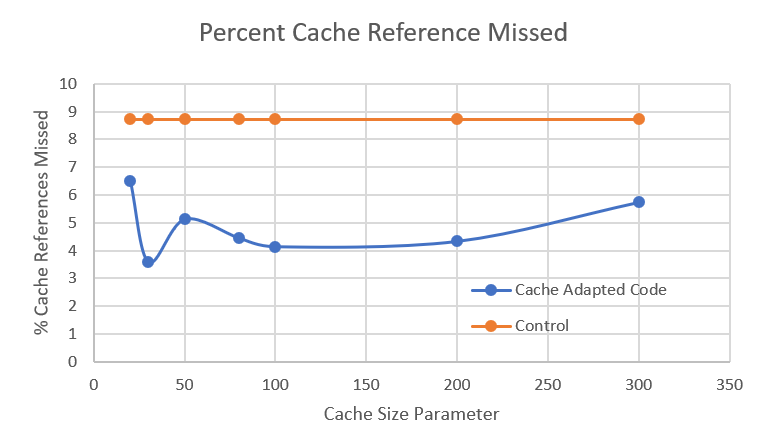
\includegraphics[width=\linewidth]{../cache_miss_plot.png}
    \caption{Cache Utilization of Staged Code.}
    \label{fig:cache_results}
  \end{figure}
  
  \begin{figure}
    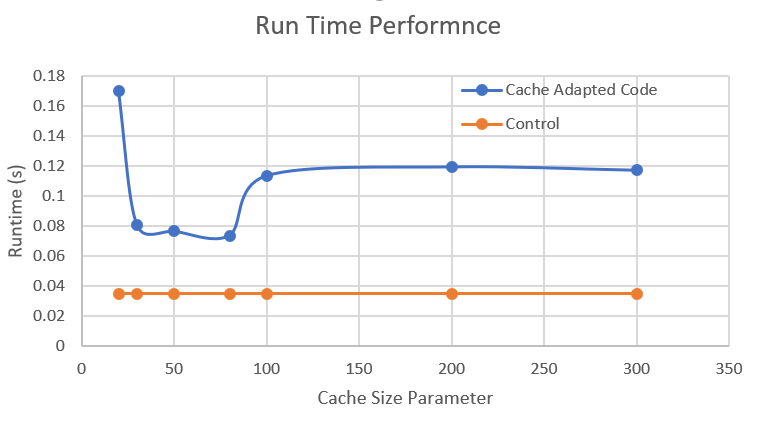
\includegraphics[width=\linewidth]{../runtime_plot.png}
  	\caption{Runtime Analysis of Staged Code.}
  	\label{fig:runtime_results}
\end{figure}

\subsection{Staging Computations}
The expression DAG contains the desired target variables that solve the Einstein equations, the sources, their corresponding dependencies, the internal nodes, which are calculate from derivates and constants, the sinks. The targets have a significant number of dependecies, the BSSN equation have dependecies on the order of 100s, such that the cache misses occur while calculating the target at each grid point in the mesh. This approach mitigates cache misses by reducing the original expression DAG into smaller sub graphs such that the number of dependencies does not exceed the cache size of the specified machine. In order to maintain correctness some of the dependencies of the original expression graph must be duplicated into multiple subgraphs. Despite computing the expression tree multiple times, the goal is to reduce runtime through increased cache efficiency.

\subsection{Subtree Isomorphism}
Once the subgraph expressions are created the goal is to order the evaluation of the sub graphs to maintain correctness and maximize cache locality. Expression subgraphs are that are a dependency of another subgraph must be computed first. If several subgraphs have no dependencies, then the subgraphs are order such that graphs with the largest Jaccard Similarity are computed one after another. In doing so variables within the cache can increase usability.  


\section{Results}
The two areas of interest are reducing cache misses and the overall runtime of the expression graphs. Figure \ref{fig:cache_results} demonstrates how the staging size affects the cache efficiency. There is a sweet spot where the staging size is large enough to leverage the entire cache while small enough to not overflow. The results presented were run on the Kingspeak Cluster at the University of Utah. The machine consits of Intel Sandy Bridge processors with 64 KB per core L1 cache, 256 KB per core L2 cache and 20 MB shared L3 cache. On the Kingspeak machines the performance was most effective with cache size of 30. Notice how all staged versions of the code were more cache efficient than the original code. 
Figure \ref{fig:runtime_results} shows the runtime analysis of the code. The runtimes were most effective when the cache utilization was the highest. However, none of the stage versions of the code were able to outperform the original code. It is hypothesized that some of the dependencies are being computed a multiple time and causing the staged code to decrease. This is a current of area of interest of improvement.


\section{Future Work}
As mentioned in the results, the original code is faster than the staged code despite the cache improvement. Within each expression subgraph, some dependencies are calculated multiple times. To reduce this the subgraphs can be staged again such that the dependencies with the largest indegree are stored in local variables for each pass.

Another area of interest is to test the autogenerated code on GPUs. GPUs have a smaller shared memory. The goal is to decrease the staging size for the code and verify that the same cache utilization is seen and determine if runtime performance increases.





\bibliographystyle{IEEEtran}
\bibliography{bssn}

\end{document}


